\documentclass[a4paper,14pt]{extarticle}
\usepackage{../../tex-shared/report-layout}

\renewcommand{\mylabnumber}{4}
\renewcommand{\mylabtitle}{Использование менеджера задач в процессе совместной работы над проектом}
\renewcommand{\mysubject}{Управление IT-проектами}
\renewcommand{\mylecturer}{Смирнова Н.Б.}

\begin{document}
\begin{titlepage}
    
    \thispagestyle{empty}
    
    \begin{center}
        
        Министерство науки и Высшего образования Российской Федерации \\
        Севастопольский государственный университет \\
        Кафедра ИС
        
        \vfill

        Отчет \\
        по лабораторной работе №\mylabnumber \\
        \enquote{\mylabtitle} \\
        по дисциплине \\
        \enquote{\MakeTextUppercase{\mysubject}}

    \end{center}

    \vspace{1cm}

    \noindent\hspace{7.5cm} Выполнил студент группы ИС/б-17-2-о \\
    \null\hspace{7.5cm} Горбенко К. Н. \\
    \null\hspace{7.5cm} Проверил \\
    \null\hspace{7.5cm} \mylecturer

    \vfill

    \begin{center}
        Севастополь \\
        \the\year{}
    \end{center}

\end{titlepage}

\section{Цель работы}
Изучить особенности использования инструментов для планирования и\\управления
задачами в процессе совместной работы над проектами.

\section{Задание на работу}
Для проекта, который был описан в 1 лабораторной работе сделать следующее:
\begin{enumerate}
    \item Разбейте проект на задачи (при необходимости – на подзадачи).
    \item Укажите исполнителей для каждой задачи (подзадачи).
    \item Расставьте приоритеты для каждой задачи (подзадачи).
    \item Составьте календарный план проекта (на выполнение проекта дается одна неделя).
\end{enumerate}

Используя, менеджер задач, создайте новый проект, над которым будет работать
ваша команда.
\begin{enumerate}
    \item Добавьте участников проекта, разослав им приглашения на email для
          участия в работе.
    \item В основном поле программы совместно добавьте задачи (подзадачи), которые вам предстоит решить.
    \item Распределите задачи между участниками проекта в соответствии с порядком выполнения.
\end{enumerate}

\begin{table}[H]
    \caption{Общая информация о проекте}
    \begin{tabular}{ | p{5.5cm} | p{11cm} | }
        \hline
        Наименование проекта & Разработка адаптивного сервиса для изучения иностранной лексики \\ \hline
        Краткое наименование проекта & Разработка адаптивного сервиса для изучения иностранной лексики \\ \hline
        Заказчик проекта & Севастопольский государственный университет \\ \hline
        Дата начала проекта & 01.05.2021 \\ \hline
        Дата окончания проекта & 31.05.2021 \\ \hline
    \end{tabular}
\end{table}

\section{Ход работы}
В результате анализа проекта выделим перечень работ по проекту и присвоим им
порядковые номера. Результаты работы заносим в таблицу \ref{tab:tasks}.

\begin{table}[H]
    \caption{Перечень работ}
    \begin{tabular}{ | C{1cm} | L{15.5cm} | }
        \hline
        № & Название события \\ \hline
        0 & Начало проекта \\ \hline
        1 & Утверждение и составление спецификаций \\ \hline
          & 1.1 Утверждение спецификаций \linebreak
            1.2 Составление технического задания \\ \hline
        2 & Проектирование архитектуры системы \\ \hline
          & 2.1 Проектирование архитектуры базы данных \linebreak
            2.2 Проектирование архитектуры административной части \linebreak
            2.3 Проектирование архитектуры пользовательской части \linebreak
            2.4 Выбор облачных поставщиков хостинга и баз данных \linebreak
            2.5 Выбор поставщиков внешних словарей \\ \hline
        3 & Разработка интерфейсов \\ \hline
        4 & Разработка дизайна и пользовательского интерфейса \\ \hline
          & 4.1 Разработка общего брендинга \linebreak
            4.2 Разработка дизайна административной части \linebreak
            4.3 Разработка дизайна пользовательской части \\ \hline
        5 & Разработка программных модулей \\ \hline
          & 5.1 Разработка БД \linebreak
            5.2 Разработка маршрутизации \linebreak
            5.3 Разработка административной части \linebreak
            5.4 Разработка пользовательской части \\ \hline
        6 & Интеграция интерфейса в программные модули \\ \hline
          & 6.1 Интеграция административной части \linebreak
            6.2 Интеграция пользовательской части \\ \hline
        7 & Разработка документации \\ \hline
        8 & Проведение тестирования \\ \hline
          & 8.1 Тестирования административной части \linebreak
            8.2 Тестирование пользовательской части \\ \hline
    \end{tabular}
    \label{tab:tasks}
\end{table}

Используя менеджер задач \code{Jira}, создадим проект и наполним его задачами:
\begin{figure}[H]
    \centering
    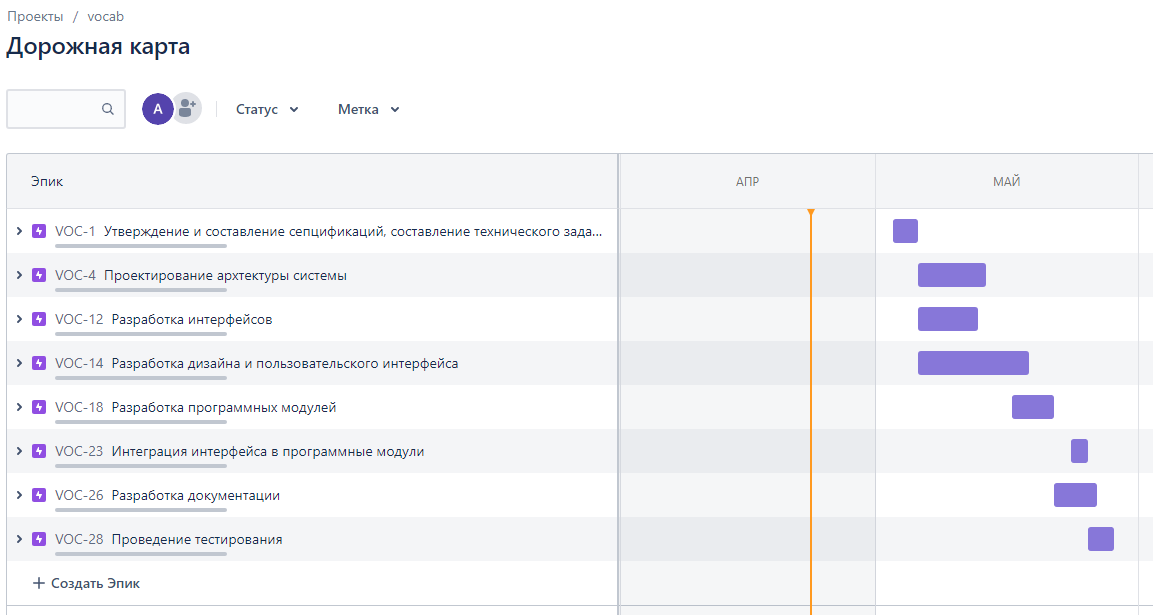
\includegraphics[width=\linewidth]{milestone}
    \caption{Список задач со сроками работ}
    \label{fig:milestone}
\end{figure}

Каждая стори состоит из нескольких подзадач, всего их 18:
\begin{figure}[H]
    \centering
    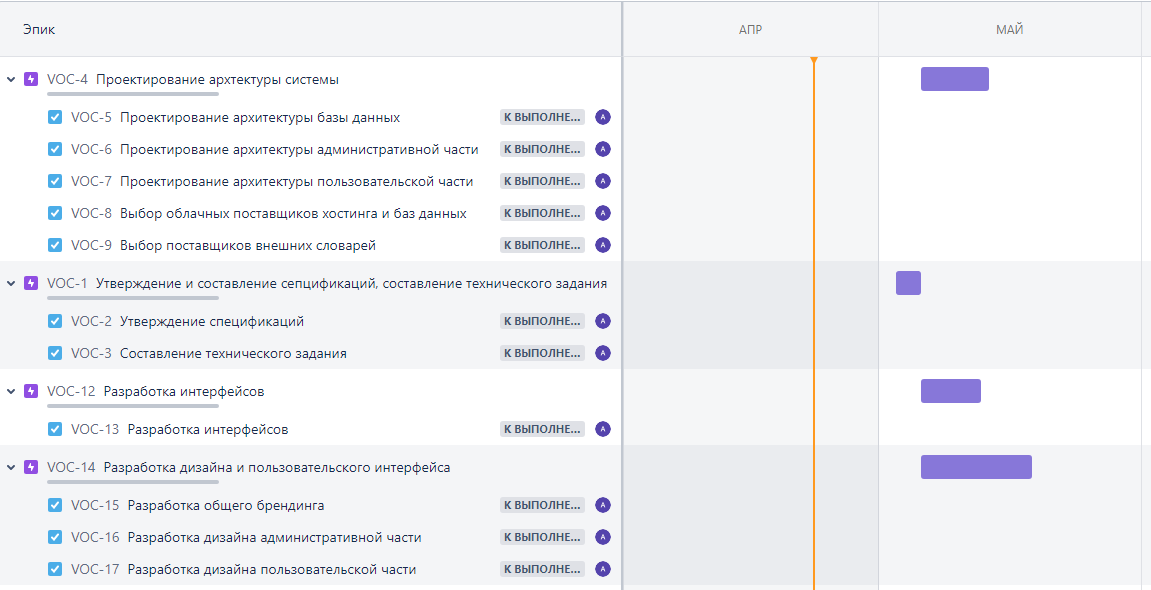
\includegraphics[width=\linewidth]{milestone-detailed}
    \caption{Разбиение задач на подзадачи}
    \label{fig:milestone-detailed}
\end{figure}

Для начала перенесем из бэклога подзадачи первой задачи:
\begin{figure}[H]
    \centering
    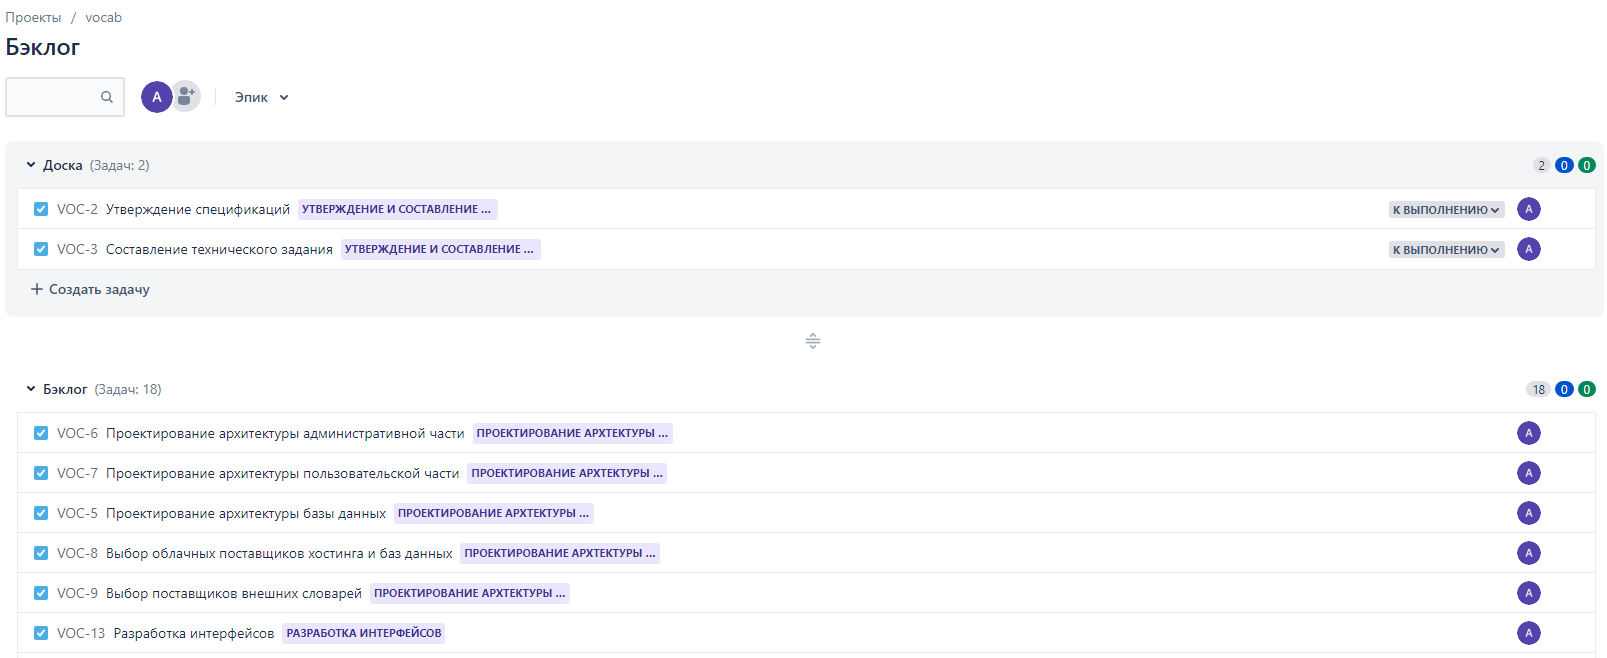
\includegraphics[width=\linewidth]{backlog}
    \caption{Бэклог}
    \label{fig:backlog}
\end{figure}

На доске изменим статусы задач:
\begin{figure}[H]
    \centering
    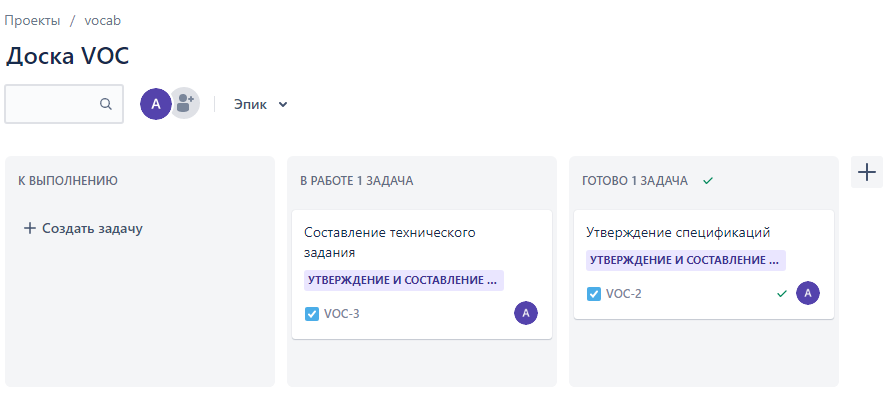
\includegraphics[width=\linewidth]{board}
    \caption{Изменение статусов задач}
    \label{fig:board}
\end{figure}

Заполним доску:
\begin{figure}[H]
    \centering
    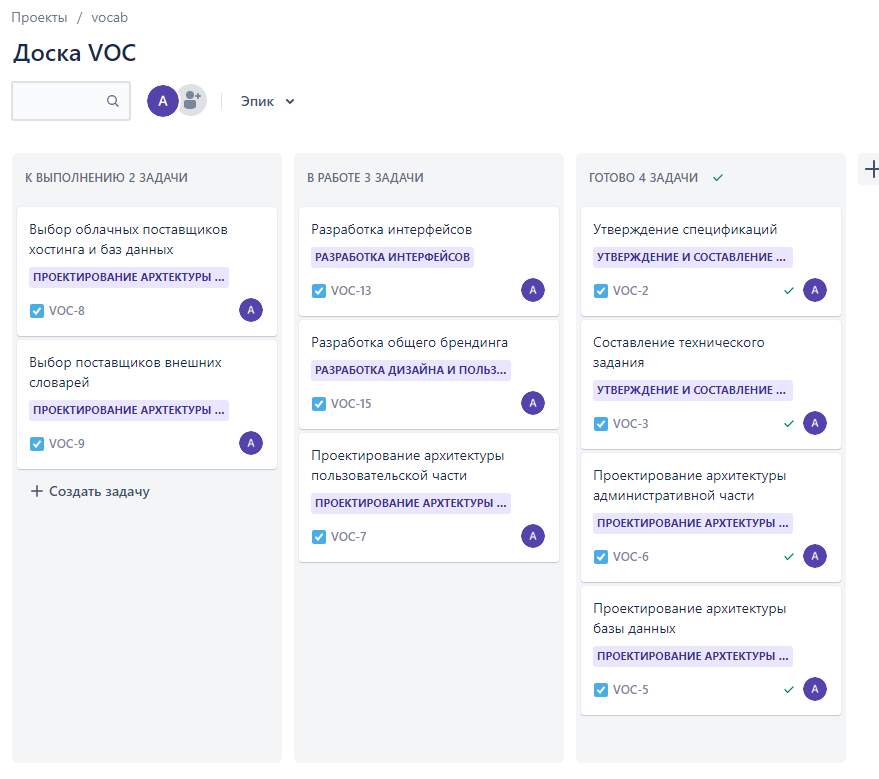
\includegraphics[width=\linewidth]{board-filled}
    \caption{Заполненная доска}
    \label{fig:board-filled}
\end{figure}

\section*{Выводы}
В ходе лабораторной работы был уточнен план проекта по разработке информационной
системы. Ознакомились с приложением Jira для управления проектами. Изучили
особенности использования инструментов для планирования и управления задачами в
процессе совместной работы над проектами.

\end{document}